\section*{Task 2: XSS and CSRF}
\subsection*{Exercises:}
\begin{enumerate}
\item The steps are as follows: 
	\begin{itemize}
		\item Open BadStore in your browser.
		\item Click "Sign Our GuestBook" on the left side of the page.
		\item In the "Your Name" field, type whatever you want.
		\item In the "Email" field, type whatever you want.
		\item In the "Comments" field, type \textit{<script>alert("1")</script>} .
		\item Click "Add Entry", the page should like this below:
		\par
		\begin{center}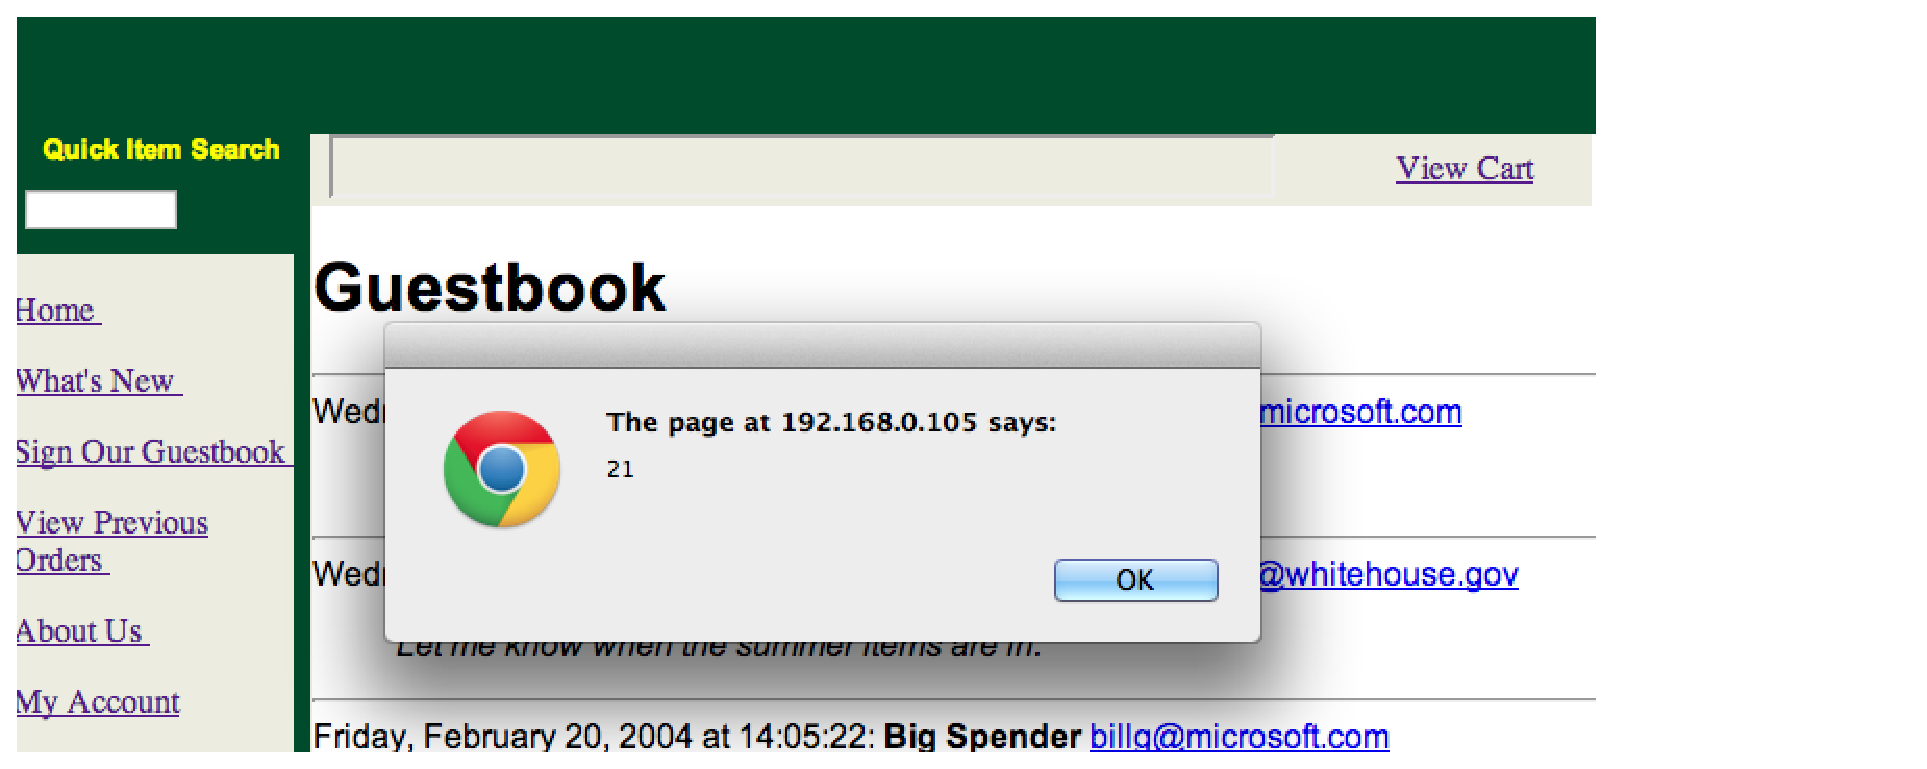
\includegraphics[height=2.5in]{xss}
		\end{center}
	\end{itemize}
	\indent Explanation: In the example, we write a piece of Javascript code in the comment area and submit it. It can work because the website has XSS vulnerability which enable us to insert and perform Javascript in the website. When it reloads, it will generate the current HTML code which contains the code we just injected. And it works as a result.
	\item To perform CSRF attacks, we need to create a custom web page contains deceived information. The function is to let user comment in the guestbook and receive countless alert. The key point is to guide victim to visit your page and click on the information. As the reason that we demonstrate it just as an example, we can  suppose that the victim will click it. Below are the steps:
	\begin{itemize}
		\item Write a simple page containing these code:
		\par
		\begin{lstlisting}[language=HTML,numbers=left,numberstyle=\tiny,columns=fullflexible,basicstyle=\footnotesize\ttfamily]
<!DOCTYPE html>
<html>
<head>
	<title>iPhone Free!</title>
</head>
<body>
	<FORM METHOD="POST" ACTION="http://10.0.2.5/cgi-bin/badstore.cgi?action=doguestbook">
		<INPUT TYPE=hidden NAME=name value="<script>for(var i=0;i<10000;i++){alert();}</script>" SIZE=30>
		<INPUT TYPE=hidden NAME=email value="1" SIZE=40>
		<TEXTAREA style="display:none" NAME=comments COLS=60 ROWS=4 value="aaa"> </TEXTAREA>
		<INPUT TYPE=submit VALUE="Get Now!">  
		<INPUT style="display:none" TYPE=reset></Center>
	</FORM>
</body>
</html>

		\end{lstlisting}
	\item The page shows like this:
	\begin{center}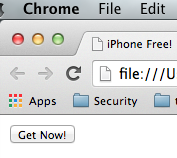
\includegraphics[height=2.5in]{csrf1}
	\end{center}
	\item Open BadStore and login in as an user.
	\item Click the "Get Now!" button in the custom page.
	\item The page will be redirected into BadStore and shows like this:
	\begin{center}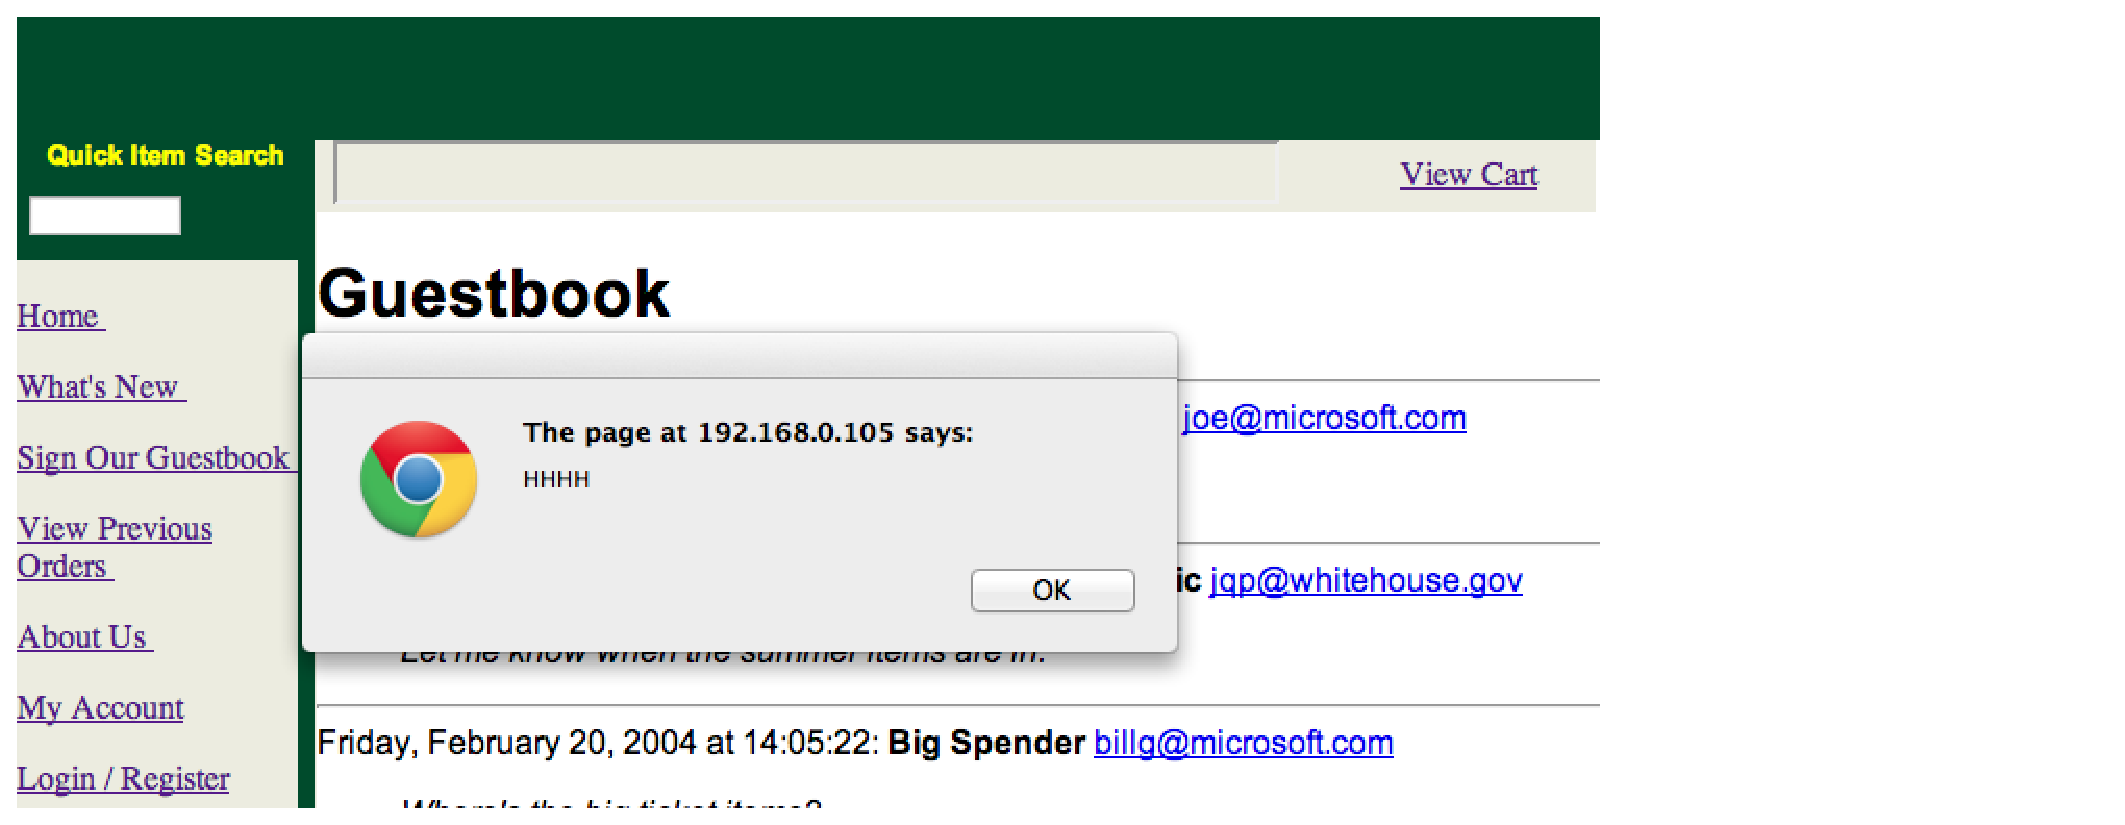
\includegraphics[height=2.5in]{csrf2}
	\end{center}
	\item The alert will repeat again and again as well as leaving many comments.
	\item Note: There might be some different performance in different browsers. i.e. Safari will operate the code after you quit it and reopen it.
	\end{itemize}
	\indent Explanation: In the example, we use a self-written page to perform CSRF attack. As mentioned above, the key point is that the attacker need to persuade the victim to visit the deceived page which contains evil code. The code can work with following reasons. First, the code will perform action in the server (BadStore) such as submitting an order or transferring money to another account. Second, the code will work because the victim doesn't close the server website. To make it clear, the cookie of the server website still exists in the browser. As a result, when the server receives the deceived request, it will think that the request is made by the victim and perform related operation.
\item
\item \highergradesonly
\item \highergradesonly
\end{enumerate}
